%%%%%%%%%%%%%%%%%%%%%%%%%%%%%%%%%%%%%%%%%
% Beamer Presentation
% LaTeX Template
% Version 1.0 (10/11/12)
%
% This template has been downloaded from:
% http://www.LaTeXTemplates.com
%
% License:
% CC BY-NC-SA 3.0 (http://creativecommons.org/licenses/by-nc-sa/3.0/)
%
%%%%%%%%%%%%%%%%%%%%%%%%%%%%%%%%%%%%%%%%%

%----------------------------------------------------------------------------------------
%	PACKAGES AND THEMES
%----------------------------------------------------------------------------------------

\documentclass[aspectratio=169]{beamer}

\mode<presentation> {

% The Beamer class comes with a number of default slide themes
% which change the colors and layouts of slides. Below this is a list
% of all the themes, uncomment each in turn to see what they look like.

%\usetheme{default}
%\usetheme{AnnArbor}
%\usetheme{Antibes}
%\usetheme{Bergen}
%\usetheme{Berkeley}
%\usetheme{Berlin}
%\usetheme{Boadilla}
%\usetheme{CambridgeUS}
%\usetheme{Copenhagen}
%\usetheme{Darmstadt}
%\usetheme{Dresden}
%\usetheme{Frankfurt}
%\usetheme{Goettingen}
%\usetheme{Hannover}
%\usetheme{Ilmenau}
%\usetheme{JuanLesPins}
%\usetheme{Luebeck}
\usetheme{Madrid}
%\usetheme{Malmoe}
%\usetheme{Marburg}
%\usetheme{Montpellier}
%\usetheme{PaloAlto}
%\usetheme{Pittsburgh}
%\usetheme{Rochester}
%\usetheme{Singapore}
%\usetheme{Szeged}
%\usetheme{Warsaw}

% As well as themes, the Beamer class has a number of color themes
% for any slide theme. Uncomment each of these in turn to see how it
% changes the colors of your current slide theme.

%\usecolortheme{albatross}
%\usecolortheme{beaver}
%\usecolortheme{beetle}
%\usecolortheme{crane}
%\usecolortheme{dolphin}
%\usecolortheme{dove}
%\usecolortheme{fly}
%\usecolortheme{lily}
%\usecolortheme{orchid}
%\usecolortheme{rose}
%\usecolortheme{seagull}
%\usecolortheme{seahorse}
%\usecolortheme{whale}
%\usecolortheme{wolverine}

%\setbeamertemplate{footline} % To remove the footer line in all slides uncomment this line
%\setbeamertemplate{footline}[page number] % To replace the footer line in all slides with a simple slide count uncomment this line

%\setbeamertemplate{navigation symbols}{} % To remove the navigation symbols from the bottom of all slides uncomment this line
}

\usepackage{graphicx} % Allows including images
\usepackage{booktabs} % Allows the use of \toprule, \midrule and \bottomrule in tables
\usepackage{pgfplots}
\usepackage{tikz}
\usepackage[demo]{tikzpeople}
\usepackage{xcolor}% or package color

\pgfplotsset{width=10cm,compat=1.9}
\usepackage{fontawesome}
\usepackage{mathtools}
\usepackage{appendixnumberbeamer}
\usepackage{subcaption}

\DeclarePairedDelimiter{\abs}{\lvert}{\rvert}

\usepgfplotslibrary{external}
\usetikzlibrary{positioning,chains}
\usepgfplotslibrary{groupplots}
\usepackage{pgfplotstable}
\usetikzlibrary{pgfplots.groupplots}
\usepackage{ifthen}
%\tikzexternalize

\newcommand{\perfplot}[3]{\begin{tikzpicture}
\begin{axis}[width=0.70\textwidth,
    height=0.6\textheight,
%    title={Performance Plot for task sequence #2},
    title style={font=\tiny},
    xlabel={Tasks},
    ylabel={Accuracy},
    symbolic x coords={#2},
    xtick=data,
    legend style={
    font=\tiny,
    cells={anchor=west},
    legend pos=outer north east,}]
    \foreach \x in {#3}
    	\addplot table [x=TASK,y=\x] {#1};
    \legend{#3}
\end{axis}
\end{tikzpicture}}

%----------------------------------------------------------------------------------------
%	TITLE PAGE
%----------------------------------------------------------------------------------------

\setbeamertemplate{headline}
{%
  \leavevmode%
  \begin{beamercolorbox}[wd=.5\paperwidth,ht=2.5ex,dp=1.125ex]{section in head/foot}%
    \hbox to .5\paperwidth{\hfil\insertsectionhead\hfil}
  \end{beamercolorbox}%
  \begin{beamercolorbox}[wd=.5\paperwidth,ht=2.5ex,dp=1.125ex]{subsection in head/foot}%
    \hbox to .5\paperwidth{\hfil\insertsubsectionhead\hfil}
  \end{beamercolorbox}%
}


\title[Catastrophic forgetting in NLP]{An investigative study of catastrophic forgetting in NLP} % The short title appears at the bottom of every slide, the full title is only on the title page

			\author[Arora]{Gaurav Arora} % Your name
\institute[Unimelb] % Your institution as it will appear on the bottom of every slide, may be shorthand to save space
{
The University of Melbourne \\ % Your institution for the title page
\medskip
Supervisors: Timothy Baldwin, Afshin Rahimi \\
}
\date{\today} % Date, can be changed to a custom date

\begin{document}

\begin{frame}
\titlepage % Print the title page as the first slide
\end{frame}


%----------------------------------------------------------------------------------------
%	PRESENTATION SLIDES
%----------------------------------------------------------------------------------------

%------------------------------------------------

	\begin{frame}
		\frametitle{Perfect Scenario}
		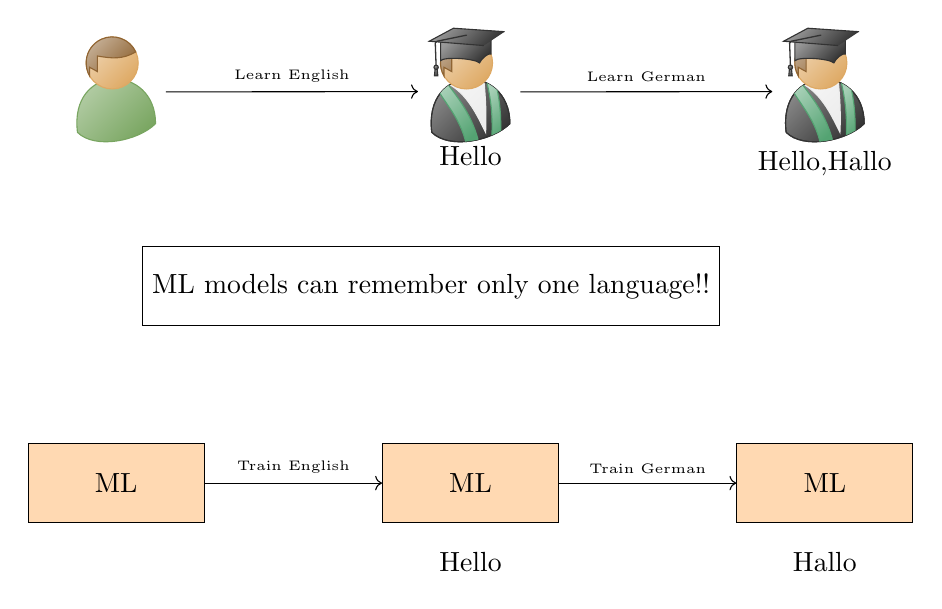
\begin{tikzpicture}
		    	\tikzstyle{ML} = [rectangle, minimum width=1cm, minimum height=1cm, text width=2cm, text centered, draw=black, fill=orange!30]
			\node[name=a,person,minimum size=1cm] (A) at (1,5) {};\pause
			\node[graduate,minimum size=1cm] (B) at (5.5,5) {Hello};
			\draw[->] (A) -- (B) node[midway,above] {\tiny Learn English}; 
			\pause
			\node[graduate,minimum size=1cm] (C) at  ( 10,5) {Hello,Hallo};
			\draw[->] (B) -- (C) node[midway,above] {\tiny Learn German}; 
			\pause
			\node[draw,minimum size=1cm] at (5,2.5) {ML models can remember only one language!!};
			\pause
			\node[ML] (A1) at (1,0) {ML};
			\pause
			\node[ML] (B1) at (5.5,0) {ML};
			\node[below of=B1] (T1) {Hello};
			\draw[->] (A1) -- (B1) node[midway,above] {\tiny Train English}; 
			\pause
			\node[ML] (C1) at  (10,0) {ML};
			\node[below of=C1] (T2) {Hallo};
			\draw[->] (B1) -- (C1) node[midway,above] {\tiny Train German}; 
		\end{tikzpicture}
	\end{frame}
	\begin{frame}
		\frametitle{Catastophic Forgetting}
		\begin{block}{Catastrophic Forgetting}
			whereby a model trained on one task is fine-tuned on a second, and in doing so, suffers a ``catastrophic'' drop in performance over the first task. 
		\end{block}
		\begin{center}
		    \begin{tikzpicture}[node distance=0 cm,outer sep = 0pt]
			\begin{axis}[
			    width=0.65\textwidth,
			    height=0.65\textheight,
			    %title={Catastrophic Forgetting},
			    xlabel={Task Sequence},
			    ylabel={Performance},
			    xtick={0,1,2,3},
			    xticklabels={Question Type, Sentiment, Grammatical}
			]

			\only<1-> \addplot[color=red,mark=square*] coordinates {(0,0.826)};
			\only<1-> \addplot[color=white] coordinates {(0,0) (1,0)};
			\only<1-> \addlegendentry{Question Type}
			\only<2-> \addplot[color=red,mark=square*] coordinates {(0,0.826)(1,0.30)};


			\end{axis}
			\end{tikzpicture}
		\end{center}
	\end{frame}
	\begin{frame}{Motivation}
	    \begin{block}{Catastrophic Forgetting}
		\centering
		Why is it important?
	    \end{block}
	\end{frame}
	\begin{frame}{Motivation}
	    \begin{block}{Tesla HydraNet: Need for Sequential Training}
		Tesla needs to retrain the whole model every time there is a misclassification for any task.
	    \end{block}
	    \begin{figure}
		\centering
		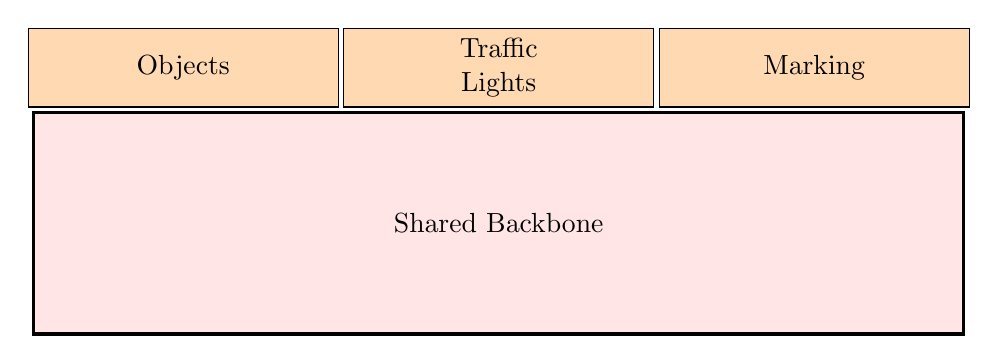
\begin{tikzpicture}[node distance=0 cm,outer sep = 1pt]
    \tikzstyle{ML} = [anchor=north east,rectangle, minimum width=11.2em, minimum height=1cm, text width=2cm, text centered, draw=black, fill=orange!30]
    \node (i1)  [anchor=south west, rectangle, align=center, draw, very thick, fill=red!10, minimum height=8em, minimum width=33.6em] {Shared Backbone};
    \node (c2)  [ML,above=of i1] {Traffic Lights};
    \node (c1)  [ML,left=of c2] {Objects};
    \node (c3)  [ML,right=of c2] {Marking};
\end{tikzpicture}

		\caption{Tesla HydraNet Model (https://www.youtube.com/watch?v=hx7BXih7zx8)}
		\label{fig:neural_arch}
	    \end{figure}
	\end{frame}

\begin{frame}{Research Objectives}
    \begin{description}
	\item[RO1:] Do current methods to reduce forgetting work for NLP tasks? \pause
	\item[RO2:] Comparing forgetting in:
	    \begin{itemize}
		\item CNN Vs LSTM
		\item Networks with different capacity 
	    \end{itemize} \pause
	\item[RO3:] Proposed methods to reduce catastrophic forgetting: 
	    \begin{itemize}
		\item Annealing Temperature schedule.
		\item Adding Task information.
	    \end{itemize}
    \end{description}
\end{frame}
\begin{frame}
	\frametitle{Tasks}
	\begin{description}
	    \onslide<1-> \item[\textbf{TREC Question classification (``TREC''):}] classify questions into \texttt{NUM, DESC, LOC, ENTY, HUM, ABBR}.
		\onslide<2-> \item[\textbf{Subjectivity (``SUBJ''):}]   binary classification of Subjectivity vs.\ Objectivity in IMDB reviews.
		\onslide<3-> \item[\textbf{Corpus of Linguistic Acceptability (``CoLA''):}]  prediction of whether a sentence is grammatical or not.
		\onslide<4-> \item[\textbf{Stanford Sentiment Treebank (``SST''):}]  fine-grained sentiment classification over five ratings (1 lowest).
	\end{description}
    \begin{block}{Continual Learning Setup}
	\begin{itemize}
		\item Tasks are trained sequentially.
		\item Tasks are trained without access to data from previous tasks.
	\end{itemize}
    \end{block}
\end{frame}
\section{Current Methods}

	\begin{frame}{RO1: Do current methods to reduce forgetting work for NLP tasks?}
	    \begin{block}{Elastic Weight Consolidation}
		Observation: Elastic Weight Consolidation reduces forgetting but hinders the learning of future tasks.
	    \end{block}\pause
	    \only<2> { \begin{figure}[h]
		\centering
		\perfplot{ewcResultTransformer.data}{CoLA,SST,TREC,SUBJ}{SUBJ|EWC,SUBJ|NORMAL}
	    \end{figure}
	    }
	    \only<3> { \begin{figure}[h]
		\centering
		%\documentclass[tikz]{standalone}
%\usetikzlibrary{positioning,chains}
%\usepackage{ifthen}

%\begin{document}

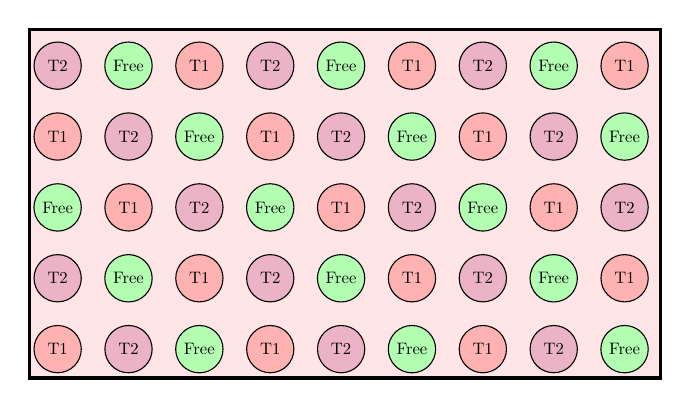
\begin{tikzpicture}[node distance=0 cm,outer sep = 1pt,transform shape,scale=0.6]
    \tikzstyle{ML0} = [anchor=north east,circle, minimum width=1cm, minimum height=1cm, text centered, draw=black, fill=red!30]
    \tikzstyle{ML1} = [anchor=north east,circle, minimum width=1cm, minimum height=1cm, text centered, draw=black, fill=purple!30]
    \tikzstyle{ML2} = [anchor=north east,circle, minimum width=1cm, minimum height=1cm, text centered, draw=black, fill=green!30]
    \node (i1) at (5.7,2.7)  [rectangle, align=center, draw, very thick, fill=red!10, minimum height=21em, minimum width=38em] {};
    \foreach \x in {0,...,8}
      \foreach \y in {0,...,4}
      {\pgfmathtruncatemacro{\label}{Mod(\x - 5 *  \y +21,3 )}
	\ifthenelse{\label = 0}
    {\node [ML0]  (\x\y) at (1.5*\x,1.5*\y) {T1}}
    {\ifthenelse{\label = 1} 
{\node [ML1]  (\x\y) at (1.5*\x,1.5*\y) {T2}}
{\node [ML2]  (\x\y) at (1.5*\x,1.5*\y) {Free}}
}
    ;}
\end{tikzpicture}

%\end{document}

	\end{figure} }
	 \end{frame}

\section{Investigative Study}
	\begin{frame}{RO2: Comparing Architectures}
	    \begin{block}{CNNs vs LSTMs}
		Observation: CNNs forget less than LSTMs due to max-pooling operation.
	    \end{block}\pause
	    \begin{figure}[h]
		\centering
		\perfplot{lstm_cnn.data}{TREC,SUBJ,CoLA,SST}{LSTM,CNN}
	    \end{figure}
	 \end{frame}
	\begin{frame}
		\frametitle{RO2: Findings from Investigative Study}
		\begin{block}{Architecture}
			CNN forgets less due to max-pooling.
		\end{block}
		\begin{block}{Network Capacity}
		    Deeper network forgets more than a shallow network.
		\end{block}

	\end{frame}

	\section{Reducing forgetting using Temperature and Task Information}
	\begin{frame}{RO3: Adding task information reduces forgetting}
	    \begin{block}{Task Information}
		Adding task information reduces forgetting.
	    \end{block}\pause
	\begin{figure}
	\centering
	    \begin{subfigure}[b]{0.45\textwidth}
	      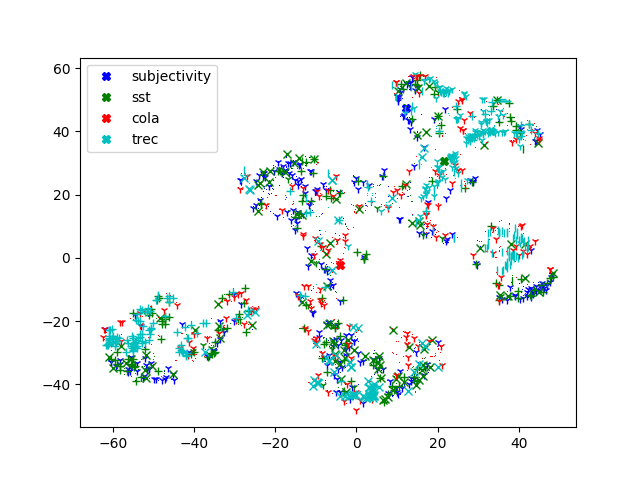
\includegraphics[scale=0.9,width=\textwidth]{lstm_normal}
	      \caption{LSTM}
	    \end{subfigure}
	    \begin{subfigure}[b]{0.45\textwidth}
	      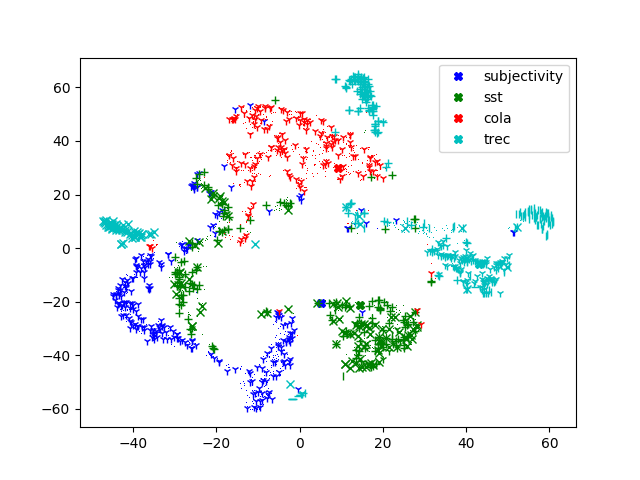
\includegraphics[scale=0.9,width=\textwidth]{lstm_task_projection}
	      \caption{LSTM with Task Information}
	    \end{subfigure}
	\end{figure}
	 \end{frame}
	\begin{frame}{RO3: Decreasing temperature schedule in softmax layer}
	    \begin{block}{Softmax Temperature}
		Temperature annealing reduces forgetting
	    \end{block}\pause
	    \begin{columns}
		\begin{column}{0.5\textwidth}
		\begin{figure}[h]
		    %\documentclass[tikz]{standalone}
%\usetikzlibrary{positioning,chains}
%\usepackage{ifthen}
%\usepackage{tikz}
%\usetikzlibrary{arrows}
%\usetikzlibrary{decorations.markings}

%\begin{document}
\tikzset{
  big arrow/.style={
    decoration={markings,mark=at position 1 with {\arrow[scale=4,#1]{>}}},
    postaction={decorate},
    shorten >=0.4pt},
  big arrow/.default=blue}

\begin{tikzpicture}[node distance=0 cm,outer sep = 1pt,transform shape,scale=0.5]
    \tikzstyle{ML0} = [anchor=north east,circle, minimum width=1cm, minimum height=1cm, text centered, draw=black, fill=red!30]
    \tikzstyle{ML1} = [anchor=north east,circle, minimum width=1cm, minimum height=1cm, text centered, draw=black, fill=purple!30]
    \tikzstyle{ML2} = [anchor=north east,circle, minimum width=1cm, minimum height=1cm, text centered, draw=black, fill=green!30]
    \tikzstyle{ML} = [anchor=north east,rectangle, minimum width=21em, minimum height=1cm, text width=2cm, text centered, draw=black, fill=orange!30]
    \node (i1) at (2.7,1.2)  [rectangle, align=center, draw, very thick, fill=red!10, minimum height=12em, minimum width=21em] {};
    \foreach \x in {0,...,4}
      \foreach \y in {0,...,2}
      {\pgfmathtruncatemacro{\label}{Mod(\x - 5 *  \y +21,3 )}
	\ifthenelse{\label = 0}
    {\node [ML0]  (\x\y) at (1.5*\x,1.5*\y) {T1}}
    {\ifthenelse{\label = 1} 
{\node [ML1]  (\x\y) at (1.5*\x,1.5*\y) {T2}}
{\node [ML2]  (\x\y) at (1.5*\x,1.5*\y) {Free}}
}
    ;}
    \node (c2)  [ML,above=of i1] {Softmax(X/0.1)};
    \node (c3) at (2.7,6.2) {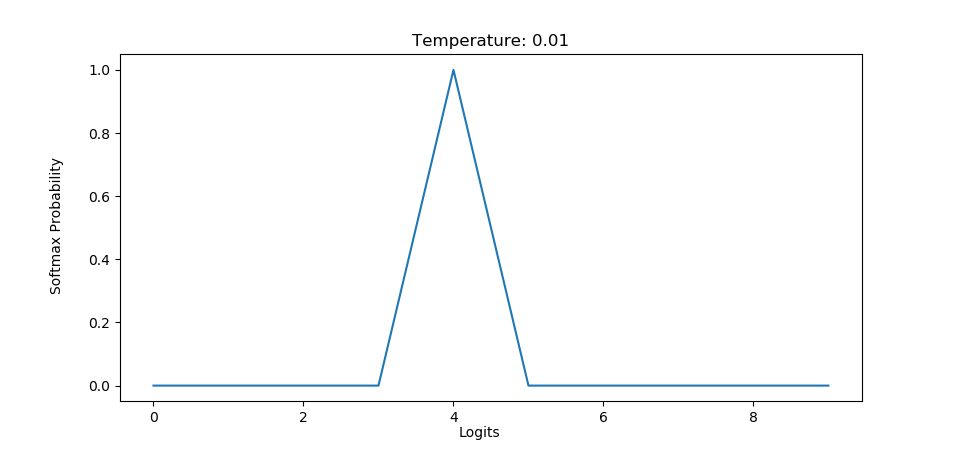
\includegraphics[width=16em]{temp_single.png}};
    \draw[red, big arrow]  (2.5,5) -- (2.5,3);

\end{tikzpicture}

%\end{document}

		    \caption{peaked output distribution}
		\end{figure}
		\end{column}
		\begin{column}{0.5\textwidth}  %%<--- here
		\begin{figure}[h]
		    %\documentclass[tikz]{standalone}
%\usetikzlibrary{positioning,chains}
%\usepackage{ifthen}
%\usepackage{tikz}
%\usetikzlibrary{arrows}
%\usetikzlibrary{decorations.markings}

%\begin{document}
\tikzset{
  big arrow/.style={
    decoration={markings,mark=at position 1 with {\arrow[scale=4,#1]{>}}},
    postaction={decorate},
    shorten >=0.4pt},
  big arrow/.default=blue}

\begin{tikzpicture}[node distance=0 cm,outer sep = 1pt,transform shape,scale=0.5]
    \tikzstyle{ML0} = [anchor=north east,circle, minimum width=1cm, minimum height=1cm, text centered, draw=black, fill=red!30]
    \tikzstyle{ML1} = [anchor=north east,circle, minimum width=1cm, minimum height=1cm, text centered, draw=black, fill=purple!30]
    \tikzstyle{ML2} = [anchor=north east,circle, minimum width=1cm, minimum height=1cm, text centered, draw=black, fill=green!30]
    \tikzstyle{ML} = [anchor=north east,rectangle, minimum width=21em, minimum height=1cm, text width=2cm, text centered, draw=black, fill=orange!30]
    \node (i1) at (2.7,1.2)  [rectangle, align=center, draw, very thick, fill=red!10, minimum height=12em, minimum width=21em] {};
    \foreach \x in {0,...,4}
      \foreach \y in {0,...,2}
      {\pgfmathtruncatemacro{\label}{Mod(\x - 5 *  \y +21,3 )}
	\ifthenelse{\label = 0}
    {\node [ML0]  (\x\y) at (1.5*\x,1.5*\y) {T1}}
    {\ifthenelse{\label = 1} 
{\node [ML1]  (\x\y) at (1.5*\x,1.5*\y) {T2}}
{\node [ML2]  (\x\y) at (1.5*\x,1.5*\y) {Free}}
}
    ;}
    \node (c2)  [ML,above=of i1] {Softmax(X/10)};
    \node (c3) at (2.7,6.2) {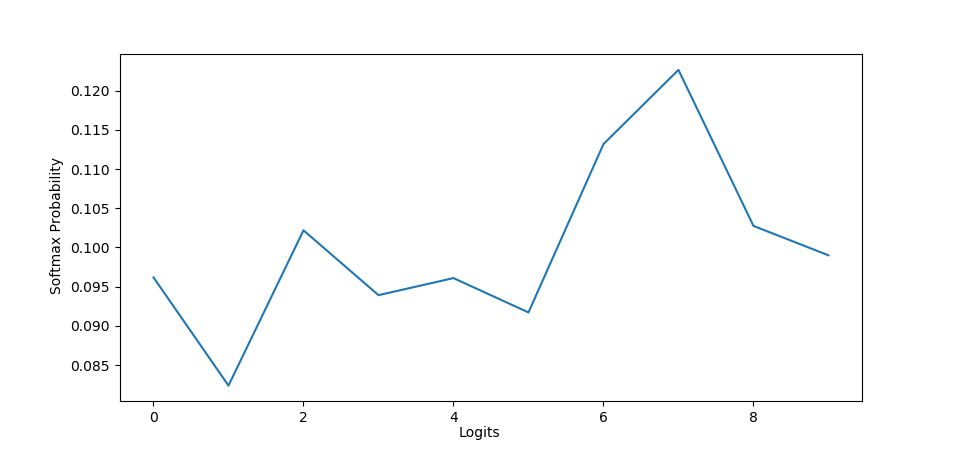
\includegraphics[width=16em]{temp_10.png}};
    \draw[red, big arrow]  (2.5,5) -- (2.5,3);
    \draw[red, big arrow]  (1,5) -- (1,3);
    \draw[red, big arrow]  (4,5) -- (4,3);

\end{tikzpicture}

%\end{document}

		    \caption{soft output distribution}
		\end{figure}
		\end{column}
		\end{columns}
	 \end{frame}
\section{Summary}
	\begin{frame}
	    \frametitle{Summary}
		\begin{block}{Continual Learning Setup}
		    \begin{itemize}
			\item Four tasks: \texttt{TREC, CoLA, SST, Subjectivity}
			\item Task trained sequentially without access to previous tasks training data.
			\item Model Architecture: \texttt{Multi-head Setup}
		    \end{itemize}
		\end{block}
		\begin{block}{Primary Findings}
		    \begin{itemize}
			\item CNN forgets less due to max-pooling.
			\item Training hard task later in the sequence is beneficial.
			\item Adding task information reduces forgetting.
			\item Temperature annealing reduces forgetting.
		    \end{itemize}
		\end{block} \pause
		   Thanks! \hfill \faGithub: gauravaror/catastrophic\_forgetting
	\end{frame}

\end{document}
